% Book pp. 129-132 (PDF pp. 130-133).  The numbering is the book's own.
\section*{Review Questions}

\begin{enumerate}
\item Use the Rational Zero Theorem to find the rational zeros of\textbf{:}
\begin{enumerate}
  \item[a.] $6x^3 - 13x^2 - 14x - 3$
  \item[b.] $5x^3 + 2x^2 - 5x - 2$
\end{enumerate}
\begin{center}
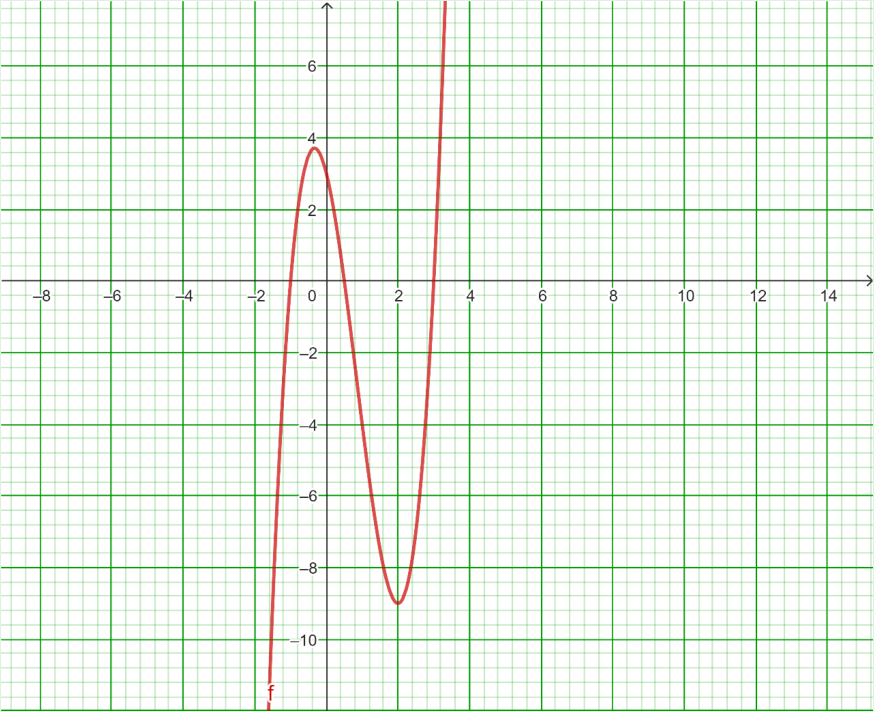
\includegraphics[width=0.7\linewidth]{figures/rq3-2.png}
\end{center}

\item Carefully, study the graph above which represents a polynomial function
f(x).
\begin{enumerate}
  \item[a.] State the zeros
  \item[b.] Find the factors
  \item[c.] State the interval on the curve.
  \item[d.] Find the polynomial function f(x)
\end{enumerate}

\item Sketch the following curves.
\begin{enumerate}
  \item[a.] $f(x) = x^3 + 2x^2 - 9x - 18$
  \item[b.] $f(x) = x^3 - 2x^2 - x + 2$
  \item[c.] $f(x) = x^3 + 3x^2 - 4x - 12$
  \item[d.] $f(x) = x^3 - 5x^2 - x + 5$
  \item[e.] $f(x) = \frac{1}{5}\left(x - 2\right)\left(x - 4\right)\left(x + 5\right)$
\end{enumerate}

\item Factorise:
\begin{enumerate}
  \item[a.] $x^3 + 5x^2 + 2x - 8$
  \item[b.] $2x^3 + 3x^2 - 17x - 30$
  \item[c.] $4x^3 - 4x^2 - 11x + 6$
  \item[d.] $6x^3 + 13x^2 - 4$
  \item[e.] $3x^3 + 16x^2 - 13x - 6$
\end{enumerate}

\item Find the zeros of the following:
\begin{enumerate}
  \item[a.] $x^3 + 4x^2 + x - 6$
  \item[b.] $2x^3 + 7x^2 - 14x + 5$
  \item[c.] $2x^3 + x^2 - 5x + 2$
  \item[d.] $4x^3 - 8x^2 - 9x + 18$
  \item[e.] $4x^3 - 4x^2 - x + 1$
  \item[f.] $4x^3 - 12x^2 + 11x - 3$
\end{enumerate}

\item Find the roots of:
\begin{enumerate}
  \item[a.] $x^3 + 6x$
  \item[b.] $2x^4 + 17x^2 + 35$
  \item[c.] $x^4 - 14x^2 + 36$
  \item[d.] $x^4 - 1$
  \item[e.] $x^3 + 27x$
\end{enumerate}
\begin{center}
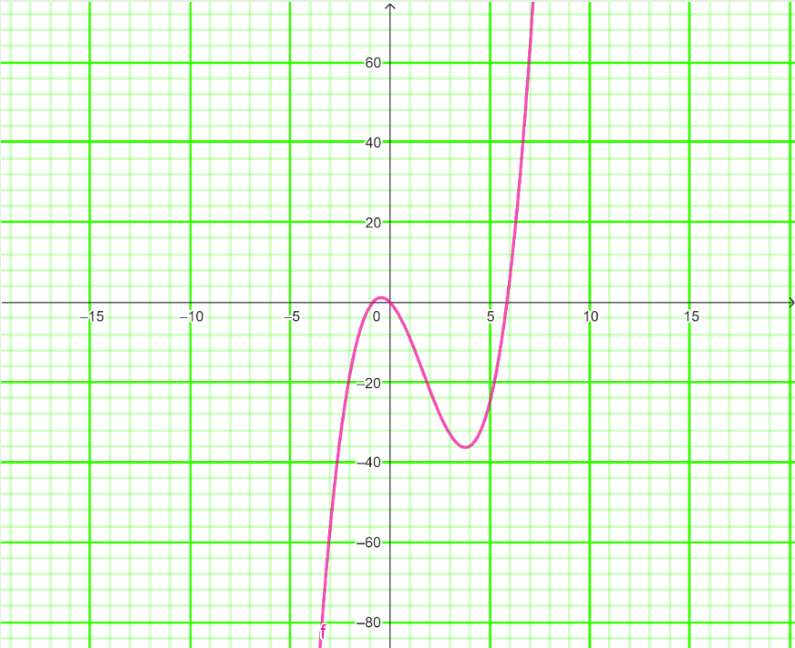
\includegraphics[width=0.65\linewidth]{figures/rq3-7.png}
\end{center}

\item Find the polynomial function f(x) as represented by the curve above.

\item $Q(x) = 10x^3 + ax^2 - 10x + b$, where $a$ and $b$ are integers, is divisible
by $(2x + 1)$. When $Q(x)$ is divided by $x + 1$, the remainder is -2.
\begin{enumerate}
  \item[a.] Find the values of a and of b
  \item[b.] find the expression for $Q(x)$ as a product of the three linear factors
\end{enumerate}

\item Given that $x_1 = 1 + \sqrt{2}\,i$ and $x_2 = 2 + 3i$ are roots of a polynomial
function $P(x)$, determine the $P(x) = 0$

\item Applying Descartes' Rule of Signs, identify the potential number of
positive and negative roots.
\begin{enumerate}
  \item[a.] $f(x) = 10x^6 - 5x^5 + 3x^4 - 6x^3 + 24x^2 - 38x$
  \item[b.] $f(x) = 19x^5 + 6x^4 + 17x^3 + 18x^2 - 38x - 70$
  \item[c.] $f(x) = x^6 - 729$
  \item[d.] $f(x) = 12x^6 + 13x^3 + 1$
  \item[e.] $f(x) = 8x^8 - 13x^4 + 100$
\end{enumerate}

\item Write down the equation having only the following roots.
\begin{enumerate}
  \item[a.] -5 , -1, 3
  \item[b.] $3, -\frac{1}{5}, -\frac{1}{3}$
  \item[c.] 2, -2, $2 + \sqrt{3}$, $2 - \sqrt{3}$
  \item[d.] 0, 1 $+$ 4i, 1- 4i
\end{enumerate}

\item Find the four roots of $y^4 + 3x^2 + 2$
\booknote[S3-16]{the polynomial mixes $y$ and $x$; the answer key treats it as
$y^4 + 3y^2 + 2$.}

\item Study the graph below and use it to answer the following questions:
\begin{enumerate}
  \item[a.] state the factors
  \item[b.] find the polynomial function
  \item[c.] how many turning points
  \item[d.] what is the relationship between the degree of the function and the
  number of turning points
\end{enumerate}
\begin{center}
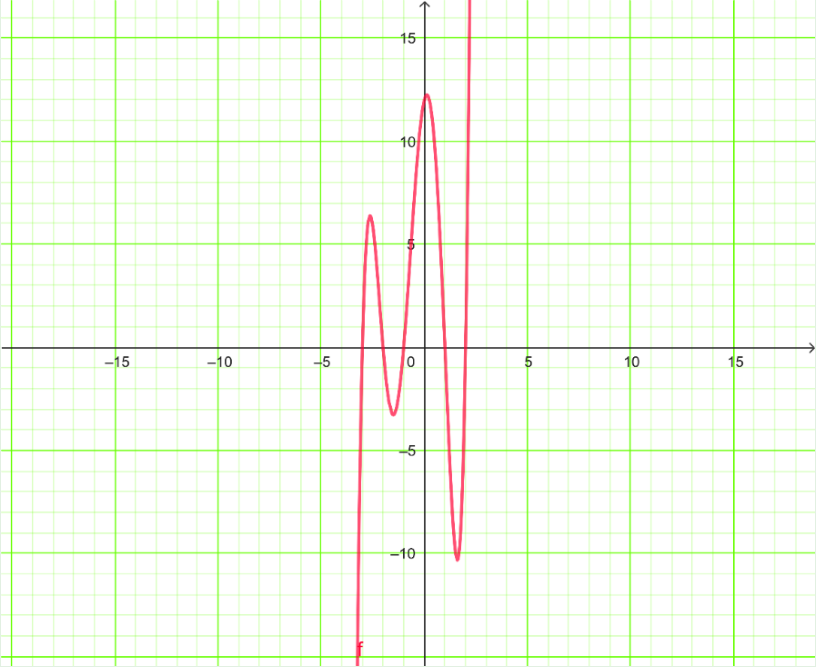
\includegraphics[width=0.65\linewidth]{figures/rq3-13.png}
\end{center}

\item A new bakery in Accra specialises in creating various types of bread. The
bakery wants the volume of a small rectangular loaf of bread to be 4 800
cm$^3$. The loaf is to be shaped like a rectangular solid. The length of the
loaf is to be 4cm longer than the width. The height of the loaf is one-half
of the width. Determine the dimensions of the loaf.
\end{enumerate}
